% Copyright (C) 2005 Thomas L. Kula
% All Rights Reserved
%
% See the file LICENSE for license terms.
\documentclass[12pt]{article}
\usepackage{graphicx}
\setlength{\paperwidth}{5.5in}
\setlength{\paperheight}{8.5in}
\setlength{\textheight}{6.45in}
\setlength{\oddsidemargin}{-0.5in}
\setlength{\evensidemargin}{-0.5in}
\setlength{\textwidth}{4.0in}
\setlength{\parindent}{0in}
\setlength{\parskip}{3mm}
\usepackage[print]{booklet} \nofiles
\source{\magstep0}{5.5in}{8.5in}
\target{\magstep0}{11in}{8.5in}
\setpdftargetpages
\begin{document}


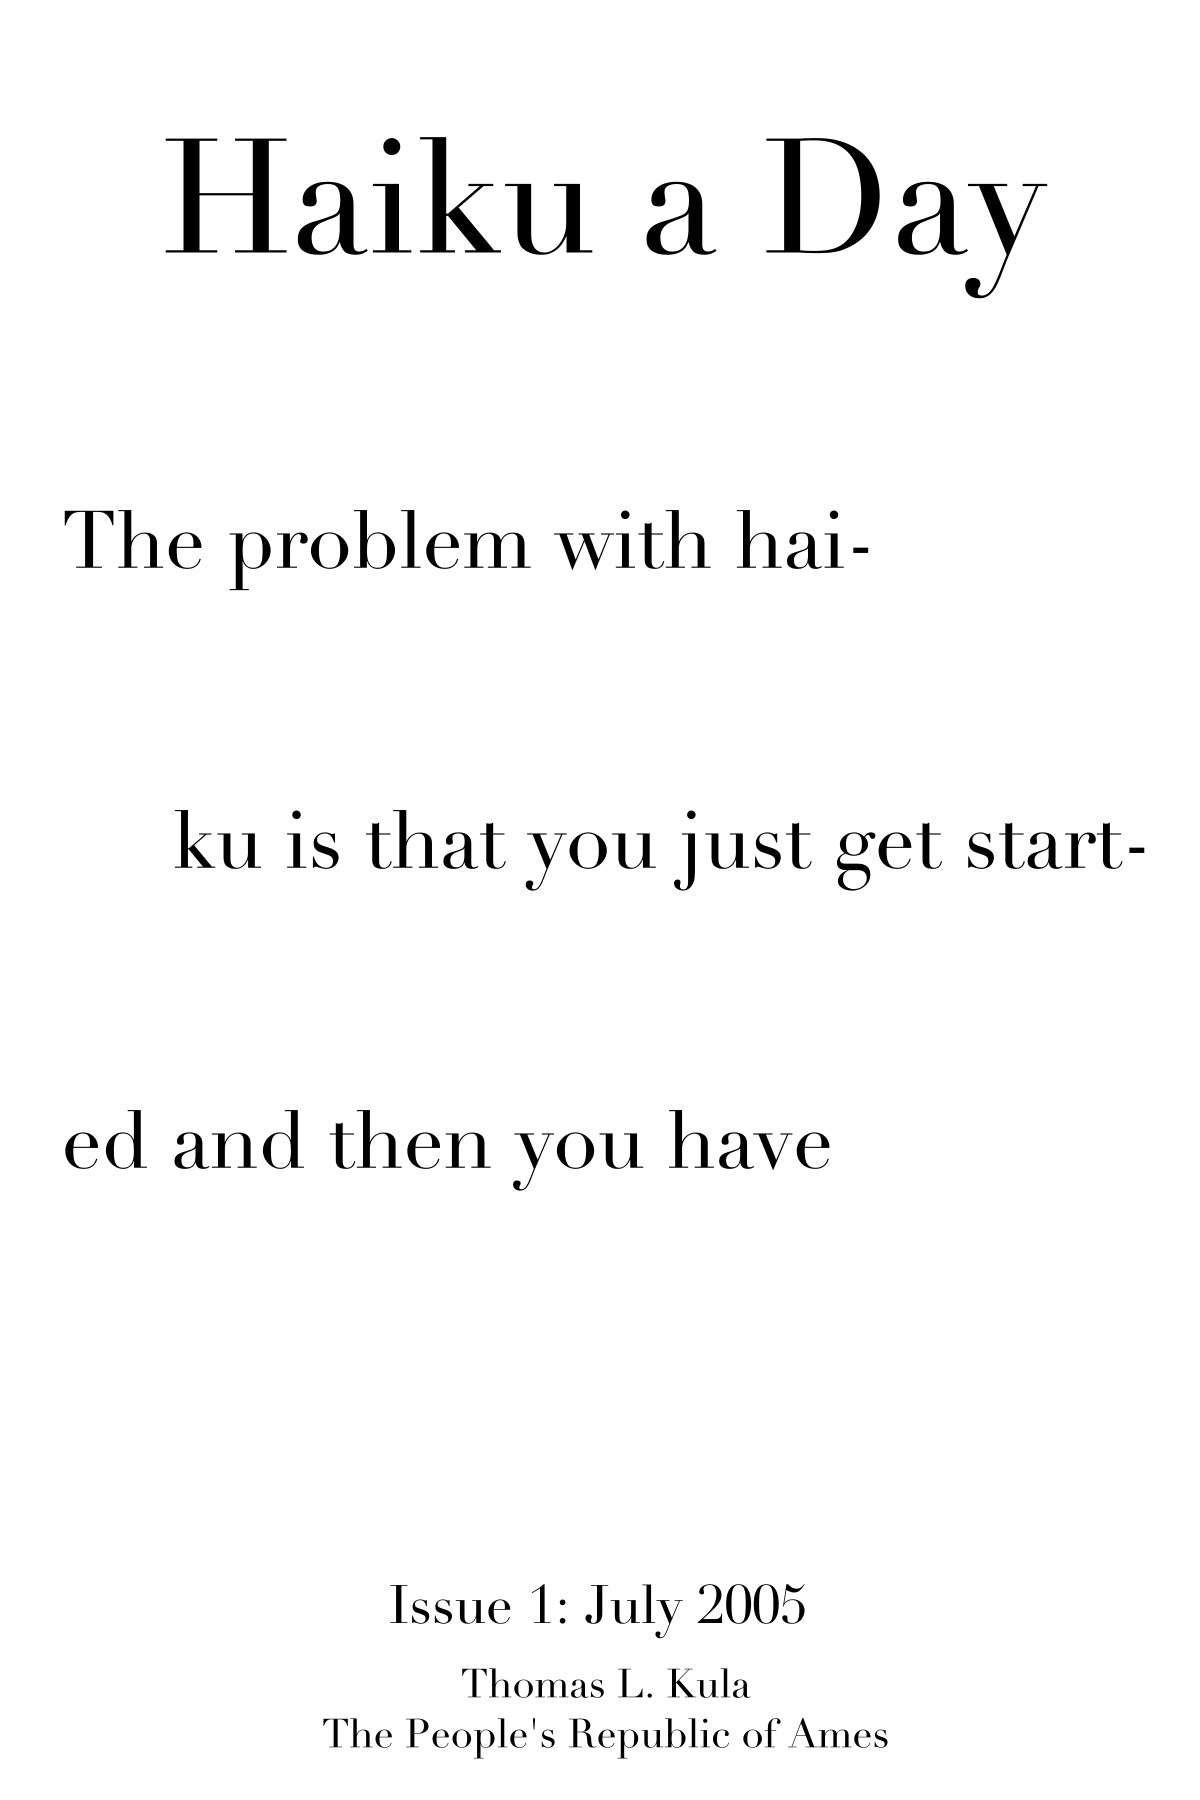
\includegraphics[width=101mm]{frontpage.png}

\newpage

In June of 2005 I was at a conference in Pittsburgh
and used the opportunity to visit one of the best
bookstores in the world (Copacetic Comics). 
There I picked up a copy
of the first of Snakepit anthology,
a collection of the daily comics Ben Snakepit
decided to start drawing back in 2000/2001.

Reading it late at night, I had the idea
to do something similar: write a haiku a
day, collect them up at the end of the month,
and send them to friends. While I don't
mean for it to be a diary (like Ben's comic
is), what you have in your hands sometimes
reflects what was happening that day, or
what I happened to be thinking about.
Not intentionally, but it happens.

Note to purists: while the Japanese poem
form known as the Haiku has more behind it
than the 5/7/5 syllable form, that's all
I'm using it for.

Enjoy.

--- Thomas

P.O. Box 1124 \\
Ames, IA 50014-1124 \\
http://kula.tproa.net/had/



\newpage
\setlength{\parskip}{1mm}

6 July 2005

Bicycling in Ames \\
It looks flat but it will make \\
Mountains from Molehills \\

7 July 2005

Cyride bus at night. \\
Haven of light in the dark \\
Takes me safely home. \\

8 July 2005

An old pair of shoes \\
They are worn, torn and broken, \\
But I can't throw them. \\

9 July 2005

Ginger beer bottle \\
Lying empty on the floor \\
Loud burps in the past. \\

10 July 2005

Haiku before sleep \\
Will I remember it at \\
The dawn of first light? \\

11 July 2005

The Jazz Department: \\
You fill the night with cool tunes \\
And some swanky beats. \\
 
\newpage

12 July 2005

The sun's rays beat down. \\
My straw hat on a hot day \\
A cool head inside. \\

13 July 2005

Longboard in corner \\
I should take you and ride, but \\
I suck at skating \\

14 July 2005

Hand blender unit \\
I use you to chop onions \\
But get onion paste \\

15 July 2005

Golden Assam tea \\
A vivid dark red color \\
Clear, malty flavor \\

16 July 2005

Washer stops spinning \\
The dryer belt is broken \\
So I hang up clothes \\

17 July 2005

A cool rain falls down \\
Heat of the day swept away \\
I enjoy the breeze. \\

\newpage

18 July 2005

Old worn out wallet \\
I've had you since the eight grade \\
You are mostly tape. \\

19 July 2005

Years of construction \\
Blasted by high explosives \\
Fall down in seconds. \\

20 July 2005

This is my boomstick \\
Bought at shop smart, shop S-Mart \\
Okay, YOU GOT THAT? \\

21 July 2005 

Water, boiling hot \\
Bleach, cleaner, scrubbing bubbles \\
My bathroom is clean \\

22 July 2005

Vegetarian \\
That word is five syllables \\
Perfect haiku line \\

23 July 2005

Titanium spork \\
A perfect addition to \\
Apocalpyse Kit. \\

\newpage

24 July 2005

Telephone rings loud \\
It's a telemarketer. \\
No one cool calls me. \\

25 July 2005

Stinky old straw hat \\
Everytime I wash you \\
You grow more worn out. \\

26 July 2005

Train goes rumbling by \\
Chugging and rumbling it goes \\
To a distant place \\

27 July 2005

Ads on building sides, \\
Fills me with an intense rage. \\
Fuck you, Ev Cochrane. \\

28 July 2005

Iowa Weather \\
If you don't like it just wait. \\
A cliche but true \\

29 July 2005

Axis of Weevil: \\
A band should do that tour. \\
It would kick some ass. \\

\newpage


30 July 2005

Moving trucks alight \\
A signal that Ames is at \\
The end of July. \\

31 July 2005

Count Infinity \\
No matter how hard you try \\
You'll never make it. \\

\newpage


\includegraphics[width=101mm]{backpage.png}

\end{document}




